%% =====================================================================
%%  Rapport de projet — Détection, analyse et correction des vulnérabilités
%%  du code généré par des Small Language Models (SLMs)
%%  INPT · Système intelligent pour la sécurité · 2026–2027
%%  Compilation : pdfLaTeX (Overleaf : Menu > Compiler = pdfLaTeX), deux passes.
%% =====================================================================
\documentclass[11pt,a4paper]{report}

% ---------- Langue, encodage, police ----------
\usepackage[utf8]{inputenc}
\usepackage[T1]{fontenc}
\usepackage[french]{babel}
\usepackage{lmodern}
\usepackage{microtype}

% ---------- Mise en page ----------
\usepackage[a4paper,top=2.5cm,bottom=2.5cm,left=2.6cm,right=2.6cm,headheight=14pt]{geometry}
\usepackage{fancyhdr}
\usepackage{titlesec}
\usepackage{setspace}
\setstretch{1.12}
\setlength{\parskip}{0.45em}

% ---------- Tableaux, figures, couleurs ----------
\usepackage{graphicx}
\graphicspath{{figures/}}
\usepackage{booktabs}
\usepackage{tabularx}
\usepackage{array}
\usepackage{multirow}
\usepackage{float}
\usepackage[font=small,labelfont=bf,labelsep=period]{caption}
\usepackage{subcaption}
\usepackage[table]{xcolor}
\usepackage{enumitem}
\setlist{itemsep=2pt,topsep=4pt}
\usepackage{amsmath}
\usepackage{listings}
\usepackage{tikz}
\usetikzlibrary{positioning,arrows.meta,shapes.multipart,fit}
\usepackage{tcolorbox}
\tcbuselibrary{skins,breakable}
\usepackage[hidelinks]{hyperref}

% ---------- Couleurs du projet (reprises de la présentation) ----------
\definecolor{accent}{HTML}{042DF5}
\definecolor{ink}{HTML}{0E0F12}
\definecolor{ink2}{HTML}{4A4D55}
\definecolor{paper}{HTML}{F2F2EE}
\definecolor{panel}{HTML}{E4E6EE}
\definecolor{okgreen}{HTML}{1A7F37}
\definecolor{badred}{HTML}{C4271B}
\hypersetup{colorlinks=true,linkcolor=accent,urlcolor=accent,citecolor=accent}

% ---------- Titres de chapitres et sections ----------
\titleformat{\chapter}[display]
  {\normalfont\bfseries\color{ink}}
  {\large\color{accent}\MakeUppercase{\chaptertitlename}~\thechapter}
  {6pt}{\Huge}[\vspace{2pt}{\color{accent}\rule{\linewidth}{1.2pt}}]
\titlespacing*{\chapter}{0pt}{-10pt}{22pt}
\titleformat{\section}{\normalfont\Large\bfseries\color{ink}}{\color{accent}\thesection}{0.8em}{}
\titleformat{\subsection}{\normalfont\large\bfseries\color{ink}}{\color{accent}\thesubsection}{0.8em}{}

% ---------- En-têtes ----------
\pagestyle{fancy}
\fancyhf{}
\fancyhead[L]{\small\color{ink2}SLM·Sec — Vulnérabilités du code généré par des SLMs}
\fancyhead[R]{\small\color{ink2}\nouppercase{\leftmark}}
\fancyfoot[C]{\small\thepage}
\renewcommand{\headrulewidth}{0.4pt}
\fancypagestyle{plain}{\fancyhf{}\fancyfoot[C]{\small\thepage}\renewcommand{\headrulewidth}{0pt}}

% ---------- Code ----------
\lstdefinestyle{py}{
  language=Python, basicstyle=\ttfamily\small, keywordstyle=\color{accent}\bfseries,
  commentstyle=\color{ink2}\itshape, stringstyle=\color{okgreen},
  numbers=left, numberstyle=\tiny\color{ink2}, numbersep=6pt,
  frame=single, rulecolor=\color{panel}, backgroundcolor=\color{paper},
  breaklines=true, showstringspaces=false, columns=fullflexible, xleftmargin=1.5em,
  inputencoding=utf8, extendedchars=true,
  literate={é}{{\'e}}1 {è}{{\`e}}1 {à}{{\`a}}1 {ê}{{\^e}}1 {ç}{{\c c}}1 {ô}{{\^o}}1 {É}{{\'E}}1}
\lstset{style=py}

% ---------- Encadrés ----------
\newtcolorbox{encadre}[1]{enhanced,breakable,colback=paper,colframe=accent,boxrule=0.6pt,
  arc=2pt,left=8pt,right=8pt,top=6pt,bottom=6pt,fonttitle=\bfseries,title={#1}}
\newcommand{\code}[1]{\texttt{\detokenize{#1}}}
\newcommand{\chiffre}[1]{\textbf{\color{accent}#1}}

% =====================================================================
\begin{document}

% ---------------------------------------------------------------------
%  Page de titre
% ---------------------------------------------------------------------
\begin{titlepage}
  \thispagestyle{empty}
  \begin{center}
    {\large\scshape Institut National des Postes et Télécommunications (INPT)}\\[2pt]
    {\normalsize Module : Système intelligent pour la sécurité}\\[1.2cm]
    {\color{accent}\rule{\linewidth}{1.4pt}}\\[0.7cm]
    {\Huge\bfseries\color{ink} Code généré, failles cachées\\[0.3cm]}
    {\LARGE Détection, analyse et correction des vulnérabilités\\ du code généré par des \emph{Small Language Models}\\[0.5cm]}
    {\color{accent}\rule{\linewidth}{1.4pt}}\\[0.8cm]
    {\large Rapport de projet}\\[1.4cm]

    \begin{minipage}[t]{0.48\linewidth}
      \raggedright
      {\small\scshape\color{ink2} Réalisé par}\\[4pt]
      Abderrahim \textsc{Attou}\\
      Aymane \textsc{El Farme}\\
      Manal \textsc{Chemlali}\\
      Youssef \textsc{Miftah}
    \end{minipage}\hfill
    \begin{minipage}[t]{0.42\linewidth}
      \raggedleft
      {\small\scshape\color{ink2} Encadré par}\\[4pt]
      Mme Meryem \textsc{Ayache}
    \end{minipage}\\[2.2cm]

    \begin{tikzpicture}
      \node[draw=accent,rounded corners=2pt,line width=0.8pt,inner sep=10pt,fill=paper,text width=12cm,align=center]{
        \small 5 SLMs \;·\; 15 prompts SecurityEval \;·\; 74 codes analysés \;·\; 20 configurations de détecteurs \;·\; 105 tentatives de correction};
    \end{tikzpicture}

    \vfill
    {\large Année universitaire 2026--2027}
  \end{center}
\end{titlepage}

% ---------------------------------------------------------------------
%  Résumé
% ---------------------------------------------------------------------
\pagenumbering{roman}
\chapter*{Résumé}
\addcontentsline{toc}{chapter}{Résumé}

Les assistants de programmation fondés sur des modèles de langage sont désormais largement utilisés. Les \emph{Small Language Models} (SLMs), qui comptent quelques milliards de paramètres, s'exécutent sur un simple GPU et préservent la confidentialité du code. Ils sont pourtant évalués presque uniquement sur la correction fonctionnelle du code qu'ils produisent (métrique pass@1), et non sur sa sécurité.

Ce projet évalue cinq SLMs open source (Qwen2.5-Coder 1.5B et 3B, StarCoder2-3B, Stable-Code-3B, TinyLlama-1.1B) dans trois rôles : \textbf{générateur} de code, \textbf{détecteur} de vulnérabilités et \textbf{correcteur}. Sur 15 prompts du jeu SecurityEval couvrant 15 catégories CWE, \chiffre{29,7\,\%} des codes générés contiennent une vulnérabilité réelle selon l'analyseur statique Bandit. Utilisés tels quels, les SLMs sont incapables de détecter les failles (F1 proche de 0) ; après un affinage QLoRA de quelques minutes sur un GPU T4, ils atteignent un F1 de \chiffre{0,67 à 0,81}, supérieur à celui de Bandit (0,64). L'ajout d'un contexte RAG à l'inférence, non vu à l'entraînement, dégrade en revanche la plupart des détecteurs. Enfin, sur 105 tentatives de correction, les contrôles automatiques en acceptent 17, mais une relecture humaine n'en confirme que \chiffre{5 (4,8\,\%)}.

Ces résultats montrent qu'un SLM spécialisé peut \emph{surveiller} efficacement le code, mais qu'il ne peut pas encore le \emph{réparer} sans supervision humaine.

\vspace{0.6em}
\noindent\textbf{Mots-clés :} Small Language Models, sécurité du code, CWE, Bandit, QLoRA, RAG, détection de vulnérabilités, correction automatique.

\chapter*{Abstract}
\addcontentsline{toc}{chapter}{Abstract}

Small Language Models (SLMs) are increasingly used as local coding assistants, yet they are mostly evaluated on functional correctness (pass@1) rather than on security. We evaluate five open-source SLMs in three roles: code generator, vulnerability detector and vulnerability fixer. On 15 SecurityEval prompts covering 15 CWE categories, 29.7\,\% of the generated programs contain a real vulnerability according to Bandit. Off-the-shelf SLMs fail as detectors (F1 close to 0), but a few minutes of QLoRA fine-tuning on a free T4 GPU raises their F1 to 0.67--0.81, above Bandit (0.64). Retrieval-augmented context added only at inference time degrades most detectors. Out of 105 repair attempts, 17 pass all automated checks, but only 5 (4.8\,\%) are confirmed by manual review. SLMs can monitor code, but cannot yet repair it without human oversight.

\tableofcontents
\listoffigures
\listoftables

\chapter*{Liste des abréviations}
\addcontentsline{toc}{chapter}{Liste des abréviations}
\begin{tabularx}{\linewidth}{@{}lX@{}}
\toprule
\textbf{Sigle} & \textbf{Signification} \\
\midrule
SLM & \emph{Small Language Model}, petit modèle de langage (ici 1 à 3 milliards de paramètres) \\
CWE & \emph{Common Weakness Enumeration}, catalogue des types de failles logicielles (MITRE) \\
LoRA & \emph{Low-Rank Adaptation}, affinage par petites matrices ajoutées au modèle \\
QLoRA & LoRA appliqué à un modèle quantifié (compressé) en 4 bits \\
RAG & \emph{Retrieval-Augmented Generation}, génération augmentée par recherche de documents \\
F1 & Moyenne harmonique de la précision et du rappel \\
MCC & Coefficient de corrélation de Matthews \\
IC 95\,\% & Intervalle de confiance à 95\,\% (estimé par bootstrap) \\
pass@1 & Proportion d'exercices réussis par la première réponse générée \\
VRAM & Mémoire du processeur graphique (GPU) \\
\bottomrule
\end{tabularx}

\cleardoublepage
\pagenumbering{arabic}

% =====================================================================
\chapter{Introduction}
% =====================================================================

\section{Contexte}
Les modèles de langage ont transformé la manière d'écrire du logiciel : complétion de code, génération de fonctions entières, explication de programmes. Parmi eux, les \emph{Small Language Models} (SLMs), de l'ordre d'un à quelques milliards de paramètres, présentent des avantages décisifs : ils s'exécutent sur un GPU grand public, ne nécessitent pas d'envoyer le code à un service externe et ont un coût quasi nul.

L'étude de référence de Hasan et al.~\cite{hasan} compare vingt SLMs sur cinq bancs d'essai (HumanEval, MBPP, Mercury, HumanEvalPack, CodeXGLUE) selon la correction fonctionnelle, l'efficacité de calcul et le support multilingue. La métrique principale y est le \textbf{pass@1} : la proportion d'exercices pour lesquels la première réponse du modèle réussit tous les tests unitaires. Cette évaluation ne dit rien de la \textbf{sécurité} du code produit.

\section{Problématique}
Un code peut être fonctionnellement correct et pourtant dangereux : un serveur web qui démarre avec un mode de débogage actif, une fonction qui désérialise des données reçues avec \code{pickle}, un mot de passe généré avec un aléa prévisible. Ces défauts sont invisibles à l'exécution. La question centrale du projet est donc :

\begin{encadre}{Question centrale}
Le code généré par les SLMs est-il sûr, et ces mêmes modèles peuvent-ils servir à détecter puis à corriger les vulnérabilités ?
\end{encadre}

\section{Questions de recherche}
\begin{description}[leftmargin=1.2cm,style=nextline]
  \item[Q1 — Génération] Les SLMs produisent-ils du code vulnérable, et dans quelles catégories CWE ?
  \item[Q2 — Détection] Un SLM peut-il détecter des vulnérabilités ? L'affinage LoRA et le RAG l'améliorent-ils par rapport à l'analyseur statique Bandit ?
  \item[Q3 — Correction] Les SLMs savent-ils corriger les vulnérabilités, dans leur propre code et dans celui des autres ?
  \item[Q4 — Taille et qualité] La taille d'un modèle ou sa performance fonctionnelle (pass@1) sont-elles liées à la sécurité de son code ?
\end{description}

\section{Contributions}
\begin{itemize}
  \item Un pipeline reproductible, exécutable sur un GPU gratuit (Google Colab, T4), qui évalue chaque SLM dans trois rôles : générateur, détecteur et correcteur.
  \item La correction de sept défauts d'une étude préliminaire, qui faussaient fortement ses conclusions.
  \item Cinq détecteurs affinés par QLoRA, comparés à Bandit avec tests statistiques.
  \item Une évaluation de la correction automatique combinant contrôles automatiques, garde-fous et relecture humaine.
\end{itemize}

\section{Organisation du rapport}
Le chapitre~\ref{chap:fondements} présente les notions utilisées. Le chapitre~\ref{chap:methodo} décrit la méthodologie et le chapitre~\ref{chap:implem} l'implémentation. Le chapitre~\ref{chap:resultats} présente les résultats, discutés au chapitre~\ref{chap:discussion}. Le chapitre~\ref{chap:conclusion} conclut.

% =====================================================================
\chapter{Fondements}\label{chap:fondements}
% =====================================================================

\section{Small Language Models}
Un modèle de langage génère du texte token par token : à chaque étape, il calcule une distribution de probabilité sur le token suivant et en choisit un. Deux paramètres de décodage contrôlent ce choix :
\begin{itemize}
  \item la \textbf{température}, qui règle le niveau d'aléa (une valeur basse, comme 0,2, favorise les tokens les plus probables) ;
  \item le \textbf{top-p} (\emph{nucleus sampling}), qui restreint le tirage aux tokens les plus probables dont la probabilité cumulée atteint $p$ (ici 0,95).
\end{itemize}
Les modèles « instruits » (\emph{instruct}) suivent des consignes en langage naturel ; les modèles « de base » se contentent de prolonger un texte, ce qui impose un mode de \emph{complétion}.

\section{Vulnérabilités et catalogue CWE}
Le catalogue CWE (\emph{Common Weakness Enumeration}), maintenu par le MITRE \cite{cwe}, attribue un identifiant à chaque type de faiblesse logicielle. Le tableau~\ref{tab:cwe} présente les familles rencontrées dans nos résultats.

\begin{table}[H]
\centering
\caption{Familles de vulnérabilités rencontrées et règles Bandit associées}
\label{tab:cwe}
\begin{tabularx}{\linewidth}{@{}llXl@{}}
\toprule
\textbf{CWE} & \textbf{Nom} & \textbf{Motif de code typique} & \textbf{Règle Bandit} \\
\midrule
CWE-502 & Désérialisation non sûre & \code{pickle.loads(data)} & B301 \\
CWE-94 / 215 & Mode debug, injection de code & \code{app.run(debug=True)} & B201 \\
CWE-259 & Mot de passe en dur & \code{password="..."} & B105, B106 \\
CWE-330 & Aléa insuffisant & \code{random.choices(...)} & B311 \\
CWE-377 & Fichier temporaire non sûr & \code{open(mktemp())} & B108, B306 \\
CWE-22 & Traversée de chemin & \code{tar.extractall()} & B202 \\
CWE-611 / 20 & XML non sûr & \code{ET.fromstring(xml)} & B314, B320 \\
CWE-89 & Injection SQL & requête construite par concaténation & B608 \\
\bottomrule
\end{tabularx}
\end{table}

\section{Analyse statique avec Bandit}
Bandit \cite{bandit} est un analyseur statique pour Python : il parcourt l'arbre syntaxique du programme, sans l'exécuter, et signale les appels dangereux connus. Chaque alerte comporte une règle (par exemple \code{B301}), une sévérité (LOW, MEDIUM, HIGH), une confiance, une ligne et, dans les versions récentes, une CWE. Bandit est rapide et déterministe, mais il ne connaît pas l'origine des données et ignore les failles logiques.

Certaines règles (B401 à B413) se déclenchent sur un simple \code{import} d'un module sensible (\code{import pickle}, \code{import subprocess}…). Importer un module n'étant pas dangereux en soi, nous les traitons comme des \textbf{alertes informatives}, distinctes des vulnérabilités réelles.

\section{Affinage QLoRA}
Réentraîner entièrement un modèle de plusieurs milliards de paramètres demande une mémoire bien supérieure à celle d'un GPU grand public. LoRA \cite{lora} fige les poids du modèle et ajoute, dans certaines couches, deux petites matrices de rang $r$ dont seul le produit est entraîné. QLoRA \cite{qlora} applique LoRA à un modèle \emph{quantifié} en 4 bits (format NF4), ce qui divise la mémoire du modèle par environ quatre. Dans ce projet, la quantification est assurée par la bibliothèque \emph{bitsandbytes} et les modules LoRA par la bibliothèque \emph{PEFT}.

\section{Génération augmentée par recherche (RAG)}
Le RAG \cite{rag} fournit au modèle, avant sa réponse, des documents pertinents retrouvés dans une base de connaissances. Les documents et la requête sont transformés en vecteurs par un modèle d'\emph{embeddings} (ici \code{bge-small-en-v1.5} \cite{bge}) ; un index FAISS \cite{faiss} retrouve les vecteurs les plus proches.

\section{Métriques d'évaluation}
\begin{itemize}
  \item \textbf{Précision} : parmi les codes signalés vulnérables, part réellement vulnérable.
  \item \textbf{Rappel} : parmi les codes vulnérables, part effectivement signalée.
  \item \textbf{F1} : moyenne harmonique de la précision et du rappel, entre 0 et 1.
  \item \textbf{MCC} : corrélation entre prédictions et vérité, robuste aux déséquilibres, entre $-1$ et $1$.
  \item \textbf{Test de McNemar} : compare deux détecteurs évalués sur les mêmes exemples.
  \item \textbf{Kappa de Cohen et de Fleiss} : accord entre détecteurs, corrigé du hasard.
  \item \textbf{pass@1} : part d'exercices réussis par la première réponse (repris de Hasan et al.~\cite{hasan}).
\end{itemize}

% =====================================================================
\chapter{Méthodologie}\label{chap:methodo}
% =====================================================================

\section{Périmètre de l'étude}
\begin{table}[H]
\centering
\caption{Périmètre de l'étude}
\label{tab:perimetre}
\begin{tabularx}{\linewidth}{@{}lX@{}}
\toprule
Langage & Python, prompts du jeu SecurityEval \cite{securityeval} \\
Modèles & 5 SLMs, de 1,1 à 3,1 milliards de paramètres \\
Vulnérabilités & 15 prompts, chacun associé à une CWE distincte \\
Détection & Bandit et détecteurs SLM (zero-shot, RAG, LoRA, LoRA + RAG) \\
Matériel & Google Colab, GPU NVIDIA T4 16 Go, calcul en fp16 \\
Hors périmètre & autres langages, exécution du code, tests fonctionnels, failles purement logiques \\
\bottomrule
\end{tabularx}
\end{table}

\section{Modèles évalués}
\begin{table}[H]
\centering
\caption{Modèles évalués (pass@1 : Hasan et al.~\cite{hasan})}
\label{tab:modeles}
\begin{tabular}{@{}llrrl@{}}
\toprule
\textbf{Modèle} & \textbf{Identifiant Hugging Face} & \textbf{Taille} & \textbf{pass@1} & \textbf{Format} \\
\midrule
Qwen2.5-Coder 1.5B & \code{Qwen/Qwen2.5-Coder-1.5B-Instruct} & 1,5 B & 0,54 & conversation \\
Qwen2.5-Coder 3B & \code{Qwen/Qwen2.5-Coder-3B-Instruct} & 3,1 B & 0,59 & conversation \\
StarCoder2 3B & \code{TechxGenus/starcoder2-3b-instruct} & 3,0 B & 0,42 & instruction \\
Stable-Code 3B & \code{stabilityai/stable-code-3b} & 2,8 B & 0,27 & complétion \\
TinyLlama 1.1B & \code{TinyLlama/TinyLlama-1.1B-Chat-v1.0} & 1,1 B & n/d & conversation \\
\bottomrule
\end{tabular}
\end{table}

Stable-Code-3B est un modèle de base, sans format d'instruction : il reçoit directement le début de code fourni par SecurityEval et en écrit la suite. TinyLlama ne figure pas dans l'étude de référence.

\section{Pipeline général}
Le projet est organisé en sept phases, une par notebook Colab (figure~\ref{fig:pipeline}).

\begin{figure}[H]
\centering
\begin{tikzpicture}[
  box/.style={draw=accent,fill=paper,rounded corners=2pt,minimum width=2.05cm,minimum height=1.1cm,align=center,font=\small},
  arr/.style={-{Stealth[length=2.2mm]},thick,color=ink2}]
  \node[box] (p0) {\textbf{00}\\Config.};
  \node[box,right=0.28cm of p0] (p1) {\textbf{01}\\Génération};
  \node[box,right=0.28cm of p1] (p2) {\textbf{02}\\Bandit};
  \node[box,right=0.28cm of p2] (p3) {\textbf{03}\\Détecteurs};
  \node[box,below=0.9cm of p3] (p4) {\textbf{04}\\Benchmark};
  \node[box,left=0.28cm of p4] (p5) {\textbf{05}\\Correction};
  \node[box,left=0.28cm of p5] (p6) {\textbf{06}\\Extras};
  \draw[arr] (p0)--(p1); \draw[arr] (p1)--(p2); \draw[arr] (p2)--(p3);
  \draw[arr] (p3)--(p4); \draw[arr] (p4)--(p5); \draw[arr] (p5)--(p6);
\end{tikzpicture}
\caption{Les sept phases du projet, un notebook par phase}
\label{fig:pipeline}
\end{figure}

\section{Génération du code (Q1)}
Les 15 prompts sont sélectionnés de façon stratifiée (une CWE distincte par prompt, avec une graine fixe) et sont identiques pour les cinq modèles. Chaque modèle produit une réponse par prompt avec les paramètres de l'étude de référence : température 0,2, top-p 0,95, 512 tokens au maximum. Le pic de mémoire et la latence sont mesurés pour chaque génération.

\paragraph{Extraction robuste.} La réponse d'un modèle peut contenir du texte autour du code, voire aucune ligne de code. Le code est extrait du bloc Markdown, puis validé par \code{ast.parse} : il doit être syntaxiquement correct et contenir au moins une véritable instruction. En cas d'échec, la génération est relancée avec une autre graine, au plus deux fois. Une réponse n'est jamais relancée parce qu'elle est vulnérable.

\section{Analyse statique (approche A)}
Chaque code exploitable est analysé par Bandit. Un code est jugé \textbf{vulnérable} s'il présente au moins une alerte réelle de sévérité MEDIUM ou HIGH. Les alertes informatives (B401 à B413) sont comptées à part ; les doublons (même règle, même ligne) sont supprimés ; la ligne et l'extrait proviennent directement du champ \code{line_number} de Bandit.

\section{Détecteur SLM (approche B)}
\subsection{Données d'entraînement}
Les détecteurs sont entraînés sur le jeu \emph{CyberNative Code Vulnerability Security DPO} \cite{cybernative}, qui fournit des paires « code vulnérable / code corrigé ». Le jeu de test SecurityEval n'est jamais utilisé pour l'entraînement ni pour la base RAG.

\begin{table}[H]
\centering
\caption{Préparation du jeu de données de détection}
\label{tab:dataset}
\begin{tabular}{@{}lr@{}}
\toprule
Paires Python au départ & 424 \\
Doublons retirés & $-52$ \\
Paires retirées (longueur, proximité avec SecurityEval) & 0 \\
\textbf{Paires conservées} & \textbf{372} \\
\midrule
Entraînement / validation / test (paires) & 297 / 37 / 38 \\
Entraînement / validation / test (exemples) & 594 / 74 / 76 \\
\bottomrule
\end{tabular}
\end{table}

Le découpage 80/10/10 est fait \textbf{par paire}, stratifié sur la CWE, pour qu'un code et sa version corrigée ne se retrouvent jamais dans deux groupes différents. Chaque groupe contient autant d'exemples vulnérables que sûrs. La CWE de référence est déduite de la description textuelle du jeu par mots-clés (classe « CWE-Other » à défaut).

\subsection{Format de sortie}
Le détecteur doit répondre par un objet JSON strict :
\begin{lstlisting}[language={},numbers=none]
{"vulnerable": true, "cwe": "CWE-502", "explanation": "<= 30 mots"}
\end{lstlisting}
La réponse est pré-remplie par \texttt{\{"vulnerable":} à l'entraînement comme à l'inférence, et la génération s'arrête à l'accolade fermante.

\subsection{Affinage QLoRA}
\begin{table}[H]
\centering
\caption{Hyperparamètres de l'affinage QLoRA}
\label{tab:qlora}
\begin{tabular}{@{}ll@{\hspace{1.5cm}}ll@{}}
\toprule
Quantification & 4 bits, NF4 & Taux d'apprentissage & $2\times10^{-4}$ \\
Calcul & fp16 & Époques & 1 \\
Rang $r$ / $\alpha$ & 16 / 32 & Lot $\times$ accumulation & $2\times8$ \\
Dropout LoRA & 0,05 & Optimiseur & paged AdamW 8 bits \\
Modules ciblés & toutes les couches linéaires & Longueur maximale & 768 tokens \\
\bottomrule
\end{tabular}
\end{table}
La perte n'est calculée que sur la réponse JSON, et non sur le code fourni en entrée.

\subsection{Base RAG}
La base de connaissances contient uniquement des données d'entraînement : les exemples vulnérables avec leur correctif, la correspondance des règles Bandit vers les CWE et de courts résumés de CWE. Pour chaque code, les trois documents les plus proches sont fournis, dans la limite d'environ 1\,200 tokens.

\subsection{Configurations comparées}
Pour chaque SLM : \textbf{base} (zero-shot), \textbf{base + RAG}, \textbf{LoRA} et \textbf{LoRA + RAG}, soit vingt configurations, toutes chargées en 4 bits pour une comparaison équitable, ainsi que Bandit.

\section{Évaluation des détecteurs}
Sur le jeu de test étiqueté (76 exemples), nous calculons l'exactitude, la précision, le rappel, le F1 et le MCC, avec des intervalles de confiance bootstrap à 95\,\%, ainsi que la justesse de la CWE sur les vrais positifs. Les configurations sont comparées deux à deux par le test de McNemar. Sur les codes générés, faute d'annotation humaine complète, la vérité terrain est une \textbf{pseudo-vérité} : un code est vulnérable si au moins 3 détecteurs sur 6 (Bandit et les cinq détecteurs LoRA) le signalent.

\section{Correction automatique (Q3)}
Les 21 codes jugés vulnérables sont soumis à chacun des cinq SLMs, soit 105 tentatives : 21 auto-corrections et 84 corrections croisées. Chaque correcteur reçoit le code, la CWE et l'explication du meilleur détecteur (Qwen2.5-Coder-3B LoRA), l'alerte Bandit et un exemple corrigé similaire retrouvé par le RAG. Une correction est d'abord jugée sur trois contrôles :
\begin{enumerate}
  \item le code est du Python valide (\code{ast.parse}) ;
  \item Bandit ne signale plus aucune alerte réelle MEDIUM ou HIGH ;
  \item le détecteur LoRA + RAG d'un \textbf{autre} modèle la juge sûre.
\end{enumerate}
En cas d'échec, une deuxième itération est lancée avec le motif du rejet. Des \textbf{garde-fous} ont été ajoutés après l'observation de faux succès : le code doit être réellement modifié (arbre syntaxique différent), conserver ses fonctions et leurs arguments, rester proche de l'original (similarité $\geq 0{,}30$), ne contenir aucun nom non défini (pyflakes) et appeler les fonctions de la bibliothèque standard avec des arguments valides. Enfin, chaque correction acceptée est \textbf{relue manuellement}.

\section{Traçabilité et reproductibilité}
Chaque étape écrit ses résultats sur Google Drive (codes générés, alertes, verdicts, corrections, revue humaine), ce qui permet de reprendre le travail après une coupure de session et de retrouver l'origine de chaque chiffre. Une graine aléatoire fixe (42), une configuration figée et un filtre anti-fuite (similarité de Jaccard $\geq 0{,}7$ avec SecurityEval) complètent le dispositif.

% =====================================================================
\chapter{Architecture et implémentation}\label{chap:implem}
% =====================================================================

\section{Architecture du système}
\begin{figure}[H]
\centering
\begin{tikzpicture}[
  col/.style={draw=accent,fill=paper,rounded corners=3pt,minimum width=4.2cm,minimum height=4.3cm,align=left,font=\small,inner sep=7pt,text width=3.8cm},
  arr/.style={-{Stealth[length=2.6mm]},very thick,color=accent}]
  \node[col] (src) {\textbf{Sources}\\\textit{Hugging Face}\\[4pt]
    • 5 modèles SLM\\• SecurityEval (évaluation)\\• CyberNative (entraînement)\\• bge-small-en-v1.5 (RAG)};
  \node[col,right=0.9cm of src,fill=panel] (cal) {\textbf{Calcul}\\\textit{Google Colab, GPU T4}\\[4pt]
    • 7 notebooks (00 à 06)\\• bibliothèque \code{slmsec.py}\\• un modèle en mémoire à la fois};
  \node[col,right=0.9cm of cal] (sto) {\textbf{Stockage}\\\textit{Google Drive}\\[4pt]
    • \code{gen/} codes\\• \code{preds/} verdicts\\• \code{adapters/} LoRA\\• \code{fix/} corrections\\• \code{results/} CSV, figures};
  \draw[arr] (src)--(cal); \draw[arr] (cal)--(sto);
\end{tikzpicture}
\caption{Architecture du système}
\label{fig:archi}
\end{figure}

Le GPU T4 ne dispose que de 16 Go de mémoire : un modèle de 3 milliards de paramètres occupe environ 6 Go en génération et jusqu'à 8,3 Go pendant l'entraînement. Chaque modèle est donc chargé, utilisé puis libéré avant le suivant. Le code commun (chargement des modèles, extraction, Bandit, détecteur, RAG, métriques, génération du rapport) est regroupé dans la bibliothèque \code{slmsec.py}.

\section{Pile technologique}
\begin{table}[H]
\centering
\caption{Technologies utilisées}
\label{tab:techno}
\begin{tabularx}{\linewidth}{@{}lX@{}}
\toprule
Transformers, Accelerate \cite{transformers} & chargement des modèles, génération, entraînement \\
PEFT, bitsandbytes & modules LoRA, quantification 4 bits, optimiseur 8 bits \\
sentence-transformers, FAISS & embeddings et recherche de voisins pour le RAG \\
Bandit, pyflakes & analyse statique, détection des noms non définis \\
datasets, pandas & chargement et manipulation des données \\
scikit-learn, statsmodels, SciPy & métriques, McNemar, kappa, corrélations \\
matplotlib & figures \\
Google Colab, Google Drive & GPU gratuit, stockage avec reprise \\
\bottomrule
\end{tabularx}
\end{table}

\section{Module de génération}
La figure~\ref{fig:cap-gen} présente la synthèse produite par le notebook 01. Quatre modèles produisent un code exploitable du premier coup pour les 15 prompts ; Stable-Code-3B a nécessité des essais supplémentaires et un prompt est resté sans code valide après trois essais. Au total, \chiffre{74 codes sur 75} sont exploitables.

\begin{figure}[H]
\centering
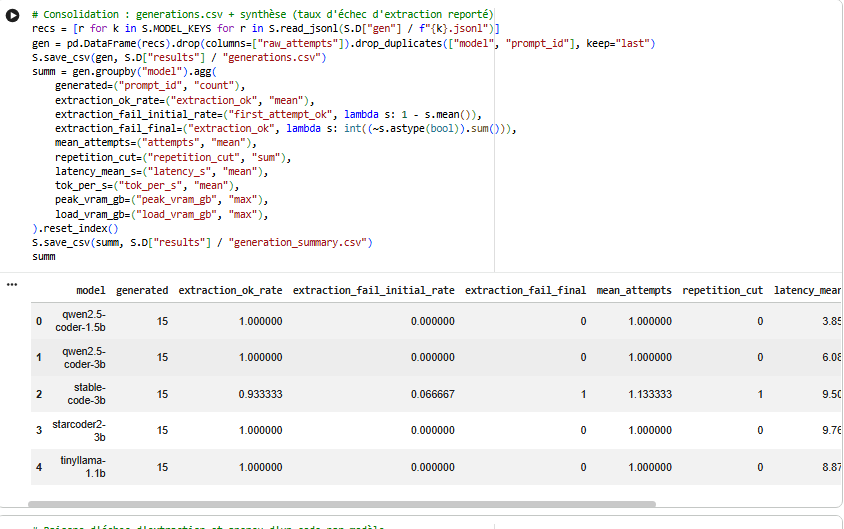
\includegraphics[width=0.92\linewidth]{01_generation.png}
\caption{Notebook 01 — synthèse de la génération (taux d'extraction, essais, latence)}
\label{fig:cap-gen}
\end{figure}

Pour Stable-Code-3B, le prompt est envoyé en mode complétion, avec des mots d'arrêt (\texttt{\#\#\#},\code{if __name__}, plusieurs lignes vides\ldots), une pénalité de répétition de 1,1 et une coupure à la première répétition d'un bloc de quatre lignes.

\section{Module d'analyse statique}
L'exemple réel ci-dessous, généré par Qwen2.5-Coder-1.5B pour le prompt \code{CWE-020_codeql_2}, illustre la distinction entre alerte informative et vulnérabilité réelle.

\begin{lstlisting}[firstnumber=1]
import base64
import pickle                                   # B403 : alerte informative

from flask import Flask, request
app = Flask(__name__)

@app.route("/profile")
def profile():
    '''Get raw_data from request ... deserialize it and return it'''
    raw_data = request.data.decode('utf-8')
    decoded_data = base64.b64decode(raw_data)
    profile_data = pickle.loads(decoded_data)   # B301 : vulnérabilité réelle (MEDIUM, CWE-502)
    return profile_data
\end{lstlisting}

\noindent L'import de \code{pickle} ne présente aucun danger ; en revanche, désérialiser des données envoyées par l'utilisateur permet d'exécuter du code arbitraire sur le serveur. Seule cette seconde alerte est comptée. La figure~\ref{fig:cap-bandit} montre le résultat de l'analyse dans le notebook 02.

\begin{figure}[H]
\centering
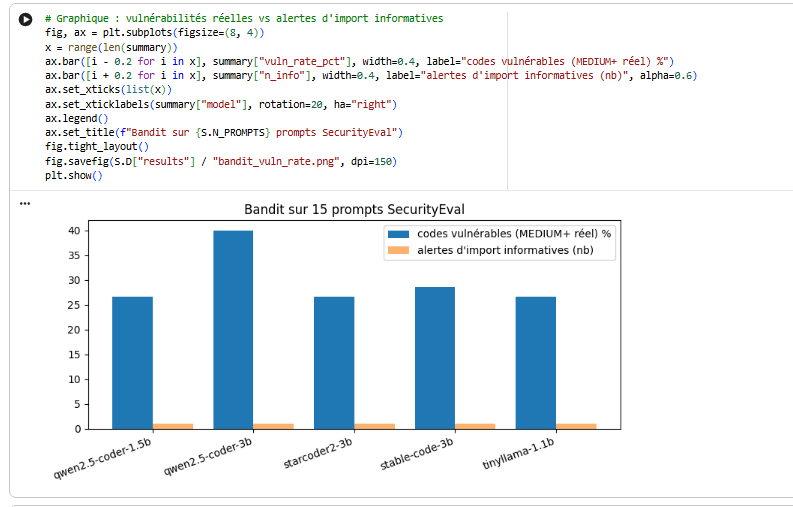
\includegraphics[width=0.85\linewidth]{02_bandit.png}
\caption{Notebook 02 — codes réellement vulnérables (bleu) et alertes d'import informatives (orange) par modèle}
\label{fig:cap-bandit}
\end{figure}

\section{Module de détection}
La configuration réelle de l'affinage QLoRA, telle qu'exécutée dans le notebook 03, est présentée à la figure~\ref{fig:cap-lora}.

\begin{figure}[H]
\centering
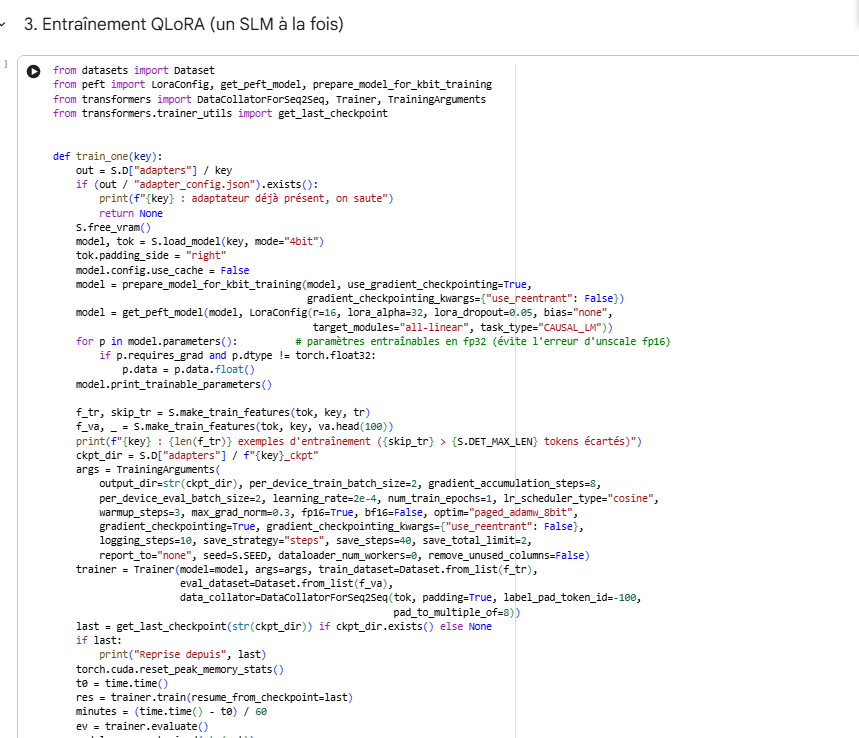
\includegraphics[width=0.82\linewidth]{04_lora.png}
\caption{Notebook 03 — configuration de l'entraînement QLoRA}
\label{fig:cap-lora}
\end{figure}

\begin{table}[H]
\centering
\caption{Journal d'entraînement des cinq détecteurs (594 exemples, 38 pas)}
\label{tab:trainlog}
\begin{tabular}{@{}lrrrr@{}}
\toprule
\textbf{Modèle} & \textbf{Perte entr.} & \textbf{Perte valid.} & \textbf{Durée (min)} & \textbf{Pic VRAM (Go)} \\
\midrule
Qwen2.5-Coder 1.5B & 0,597 & 0,388 & 3,8 & 5,76 \\
Qwen2.5-Coder 3B & 0,586 & 0,364 & 5,8 & 8,13 \\
StarCoder2 3B & 0,623 & 0,412 & 5,6 & 7,40 \\
Stable-Code 3B & 0,551 & 0,375 & 5,8 & 8,34 \\
TinyLlama 1.1B & 0,571 & 0,394 & 2,9 & 6,95 \\
\bottomrule
\end{tabular}
\end{table}

\section{Module de correction}
Le bilan automatique de la correction, par correcteur, est présenté à la figure~\ref{fig:cap-fix}. Les garde-fous décrits à la section précédente ont été motivés par des cas réels : une « correction » qui supprimait une simple ligne vide, une autre qui utilisait \code{io.BytesIO} sans importer \code{io}, une troisième qui appelait \code{secrets.choice(..., k=16)}, fonction qui n'accepte pas l'argument \code{k}.

\begin{figure}[H]
\centering
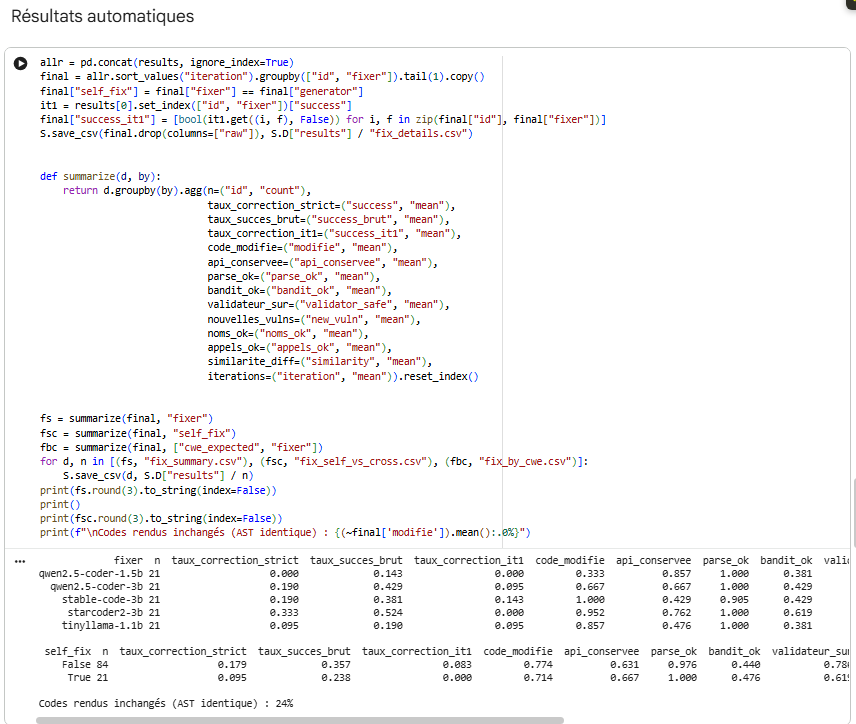
\includegraphics[width=0.85\linewidth]{05_correction.png}
\caption{Notebook 05 — résultats automatiques de la correction par correcteur}
\label{fig:cap-fix}
\end{figure}

\section{Corrections apportées à l'étude préliminaire}
Avant les expériences, nous avons audité une première version de l'étude et corrigé sept défauts (tableau~\ref{tab:bugs}). Le plus révélateur concerne Qwen2.5-Coder-3B : l'ancien rapport lui attribuait 0\,\% de code vulnérable, uniquement parce que son code n'était pas extrait ; une fois l'extraction corrigée, ce taux atteint 40\,\%.

\begin{table}[H]
\centering
\caption{Défauts de l'étude préliminaire et corrections}
\label{tab:bugs}
\begin{tabularx}{\linewidth}{@{}cXX@{}}
\toprule
\textbf{\#} & \textbf{Défaut} & \textbf{Correction} \\
\midrule
1 & Une phrase sans code comptée comme code sain & Validation par \code{ast.parse}, jusqu'à deux régénérations \\
2 & Stable-Code bouclait sur \og \#\#\# Instruction \fg & Mode complétion, mots d'arrêt, coupure des répétitions \\
3 & Toutes les alertes placées à la ligne 1 & Ligne réelle fournie par Bandit, doublons supprimés \\
4 & Imports comptés comme vulnérabilités & Alertes B401--B413 traitées comme informatives \\
5 & Observations identiques pour tous les modèles & Observations générées à partir des données \\
6 & Trois CWE seulement & 15 prompts couvrant 15 CWE distinctes \\
7 & Accents corrompus dans les fichiers & Écriture systématique en UTF-8 \\
\bottomrule
\end{tabularx}
\end{table}

% =====================================================================
\chapter{Résultats}\label{chap:resultats}
% =====================================================================

\section{Protocole expérimental}
L'expérience porte sur 5 modèles, 75 codes générés (74 exploitables), 76 exemples de test étiquetés, 20 configurations de détecteurs et 105 tentatives de correction.

\section{Q1 — Sécurité du code généré}
\begin{table}[H]
\centering
\caption{Vulnérabilités détectées par Bandit dans le code généré (alertes réelles MEDIUM+)}
\label{tab:gen}
\begin{tabular}{@{}lccccc@{}}
\toprule
\textbf{Modèle} & \textbf{Vulnérables} & \textbf{Taux} & \textbf{HIGH / MED. / LOW} & \textbf{Latence (s)} & \textbf{VRAM (Go)} \\
\midrule
Qwen2.5-Coder 1.5B & 4 / 15 & 26,7\,\% & 2 / 3 / 2 & 3,9 & 3,1 \\
\rowcolor{panel} Qwen2.5-Coder 3B & 6 / 15 & \textbf{40,0\,\%} & 3 / 3 / 3 & 6,1 & 6,2 \\
StarCoder2 3B & 4 / 15 & 26,7\,\% & 2 / 4 / 3 & 9,8 & 6,1 \\
Stable-Code 3B & 4 / 14 & 28,6\,\% & 0 / 5 / 6 & 9,5 & 5,8 \\
TinyLlama 1.1B & 4 / 15 & 26,7\,\% & 2 / 3 / 4 & 8,9 & 2,2 \\
\midrule
\textbf{Total} & \textbf{22 / 74} & \textbf{29,7\,\%} & & & \\
\bottomrule
\end{tabular}
\end{table}

\begin{figure}[H]
\centering
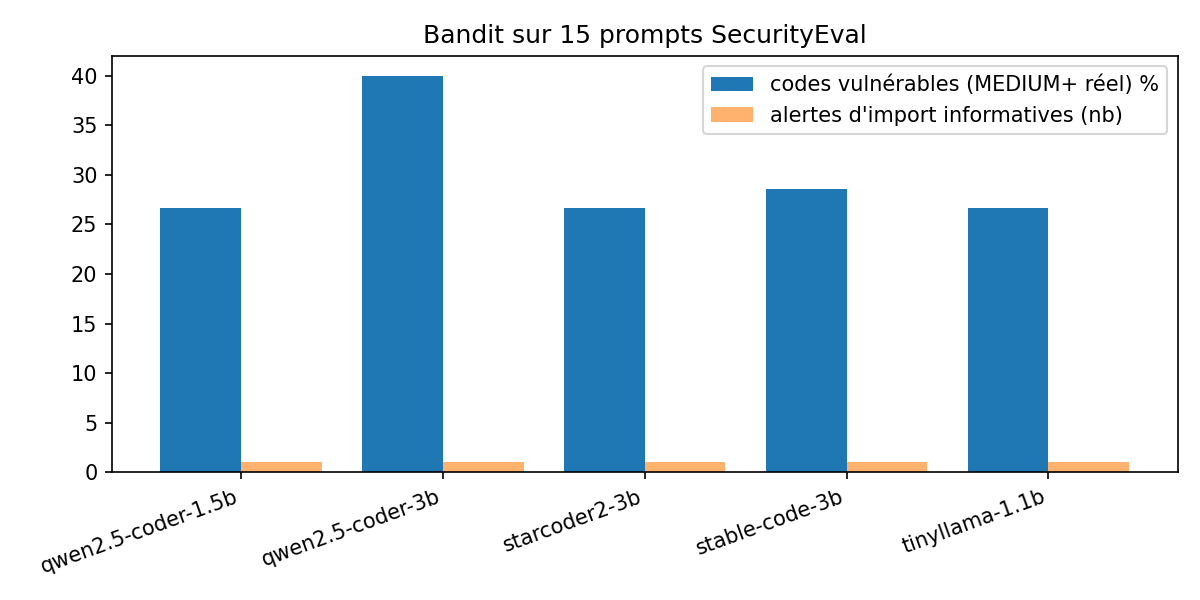
\includegraphics[width=0.78\linewidth]{bandit_vuln_rate.png}
\caption{Taux de codes vulnérables par modèle (Bandit, 15 prompts SecurityEval)}
\label{fig:bandit}
\end{figure}

Tous les modèles produisent du code vulnérable. Les failles les plus fréquentes relèvent de \og réflexes d'API \fg : désérialisation avec \code{pickle}, mode debug de Flask, module \code{random} pour des secrets, mots de passe écrits en dur. Les prompts CWE-020, CWE-022, CWE-259 et CWE-330 déclenchent des alertes Bandit chez les cinq modèles. Avec 15 codes par modèle, un code de différence représente toutefois près de 7 points : les écarts entre modèles doivent être interprétés avec prudence.

\section{Q2 — Détection des vulnérabilités}
\begin{table}[H]
\centering
\caption{Score F1 des détecteurs sur le test étiqueté (76 exemples)}
\label{tab:f1}
\begin{tabular}{@{}lcccc@{}}
\toprule
\textbf{Détecteur} & \textbf{Base} & \textbf{Base + RAG} & \textbf{LoRA} & \textbf{LoRA + RAG} \\
\midrule
Qwen2.5-Coder 1.5B & 0,00 & 0,00 & 0,67 & \textbf{0,77} \\
Qwen2.5-Coder 3B & 0,04 & 0,10 & \textbf{0,81} & 0,69 \\
StarCoder2 3B & 0,00 & 0,00 & \textbf{0,75} & 0,67 \\
Stable-Code 3B & 0,10 & 0,00 & \textbf{0,78} & 0,49 \\
TinyLlama 1.1B & 0,00 & 0,00 & \textbf{0,78} & 0,05 \\
\midrule
\textit{Bandit (référence)} & \multicolumn{4}{c}{\textit{0,64}} \\
\bottomrule
\end{tabular}
\end{table}

\begin{table}[H]
\centering
\caption{Détail de la configuration LoRA et de Bandit}
\label{tab:lora}
\begin{tabular}{@{}lcccccc@{}}
\toprule
\textbf{Détecteur} & \textbf{Exact.} & \textbf{Préc.} & \textbf{Rappel} & \textbf{F1 [IC 95\,\%]} & \textbf{MCC} & \textbf{CWE juste} \\
\midrule
Qwen2.5-Coder 1.5B & 0,70 & 0,74 & 0,61 & 0,67 [0,52 -- 0,79] & 0,40 & 100\,\% \\
\rowcolor{panel} Qwen2.5-Coder 3B & 0,80 & 0,77 & 0,87 & 0,81 [0,71 -- 0,89] & 0,61 & 88\,\% \\
StarCoder2 3B & 0,75 & 0,74 & 0,76 & 0,75 [0,64 -- 0,85] & 0,50 & 79\,\% \\
Stable-Code 3B & 0,75 & 0,69 & 0,89 & 0,78 [0,67 -- 0,87] & 0,52 & 85\,\% \\
TinyLlama 1.1B & 0,78 & 0,77 & 0,79 & 0,78 [0,67 -- 0,88] & 0,55 & 76\,\% \\
Bandit & 0,59 & 0,57 & 0,71 & 0,64 [0,51 -- 0,74] & 0,19 & 41\,\% \\
\bottomrule
\end{tabular}
\end{table}

\begin{figure}[H]
\centering
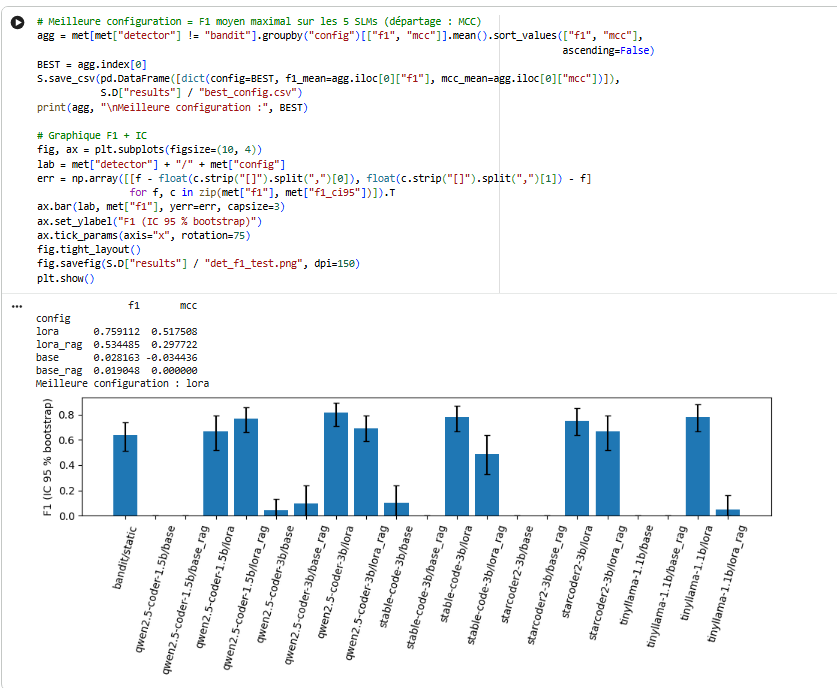
\includegraphics[width=0.9\linewidth]{03_cwe.png}
\caption{Notebook 04 — F1 par détecteur et configuration avec intervalles de confiance ; meilleure configuration : LoRA}
\label{fig:cap-f1}
\end{figure}

\paragraph{Analyse.}
\begin{itemize}
  \item \textbf{Les modèles de base ne détectent pas} : ils répondent presque toujours \og sûr \fg, d'où un F1 proche de 0.
  \item \textbf{L'affinage LoRA est décisif} : le gain par rapport au modèle de base est significatif pour les cinq modèles (McNemar, $p \leq 0{,}02$).
  \item \textbf{LoRA dépasse Bandit} pour les cinq modèles, de façon significative pour quatre d'entre eux ($p < 0{,}04$ ; Qwen2.5-Coder 1.5B : $p = 0{,}19$).
  \item \textbf{Le RAG n'aide qu'un modèle} (Qwen2.5-Coder 1.5B) et dégrade les autres, significativement pour Qwen2.5-Coder 3B ($p = 0{,}001$) et TinyLlama ($p = 0{,}002$). Le contexte n'ayant pas été vu pendant l'entraînement, il décale la distribution d'entrée et rend certains détecteurs trop alarmistes ou muets.
  \item Toutes les configurations produisent un JSON valide (0\,\% de réponses inutilisables).
\end{itemize}

\section{Rôles échangés : générateurs et détecteurs}
\begin{figure}[H]
\centering
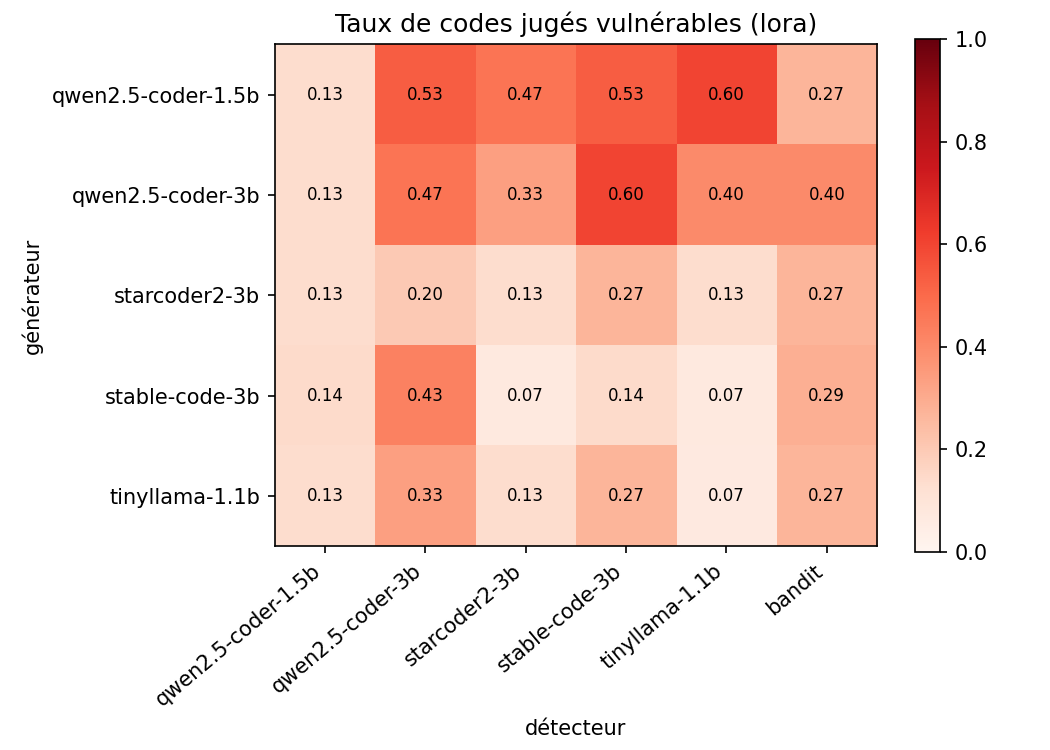
\includegraphics[width=0.72\linewidth]{cross_matrix.png}
\caption{Taux de codes jugés vulnérables, par générateur (lignes) et par détecteur (colonnes), configuration LoRA}
\label{fig:cross}
\end{figure}

L'accord entre les six détecteurs est modéré (kappa de Fleiss 0,36 ; kappa de Cohen moyen 0,35) : ils ne signalent pas les mêmes codes. Trois détecteurs se montrent plus indulgents envers leur propre code : StarCoder2 (13\,\% contre 25\,\% pour le code des autres), Stable-Code (14\,\% contre 42\,\%) et TinyLlama (7\,\% contre 31\,\%) ; Qwen2.5-Coder 3B fait exception (47\,\% contre 37\,\%).

\begin{figure}[H]
\centering
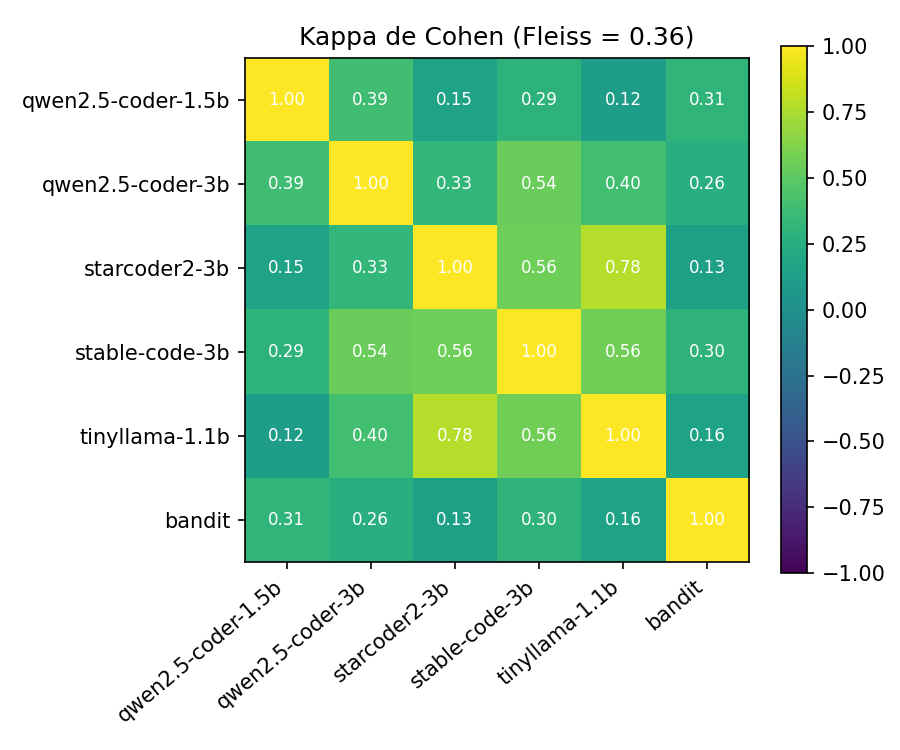
\includegraphics[width=0.6\linewidth]{kappa_cohen.png}
\caption{Accord deux à deux entre détecteurs (kappa de Cohen)}
\label{fig:kappa}
\end{figure}

\section{Q3 — Correction automatique}
\begin{table}[H]
\centering
\caption{Résultats de la correction par correcteur (21 tentatives chacun)}
\label{tab:fix}
\begin{tabular}{@{}lcccc@{}}
\toprule
\textbf{Correcteur} & \textbf{Succès brut} & \textbf{Succès strict} & \textbf{Validés (humain)} & \textbf{Taux réel} \\
\midrule
Qwen2.5-Coder 1.5B & 14\,\% & 0 & 0 & 0,0\,\% \\
Qwen2.5-Coder 3B & 43\,\% & 4 & 2 & 9,5\,\% \\
StarCoder2 3B & 52\,\% & 7 & 1 & 4,8\,\% \\
Stable-Code 3B & 38\,\% & 4 & 2 & 9,5\,\% \\
TinyLlama 1.1B & 19\,\% & 2 & 0 & 0,0\,\% \\
\midrule
\textbf{Total (105)} & \textbf{33\,\% (35)} & \textbf{17} & \textbf{5} & \textbf{4,8\,\%} \\
\bottomrule
\end{tabular}
\end{table}

\begin{figure}[H]
\centering
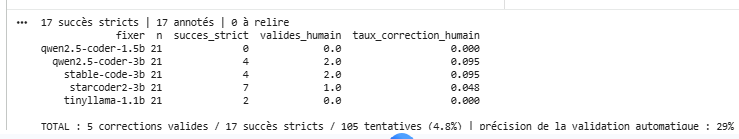
\includegraphics[width=0.92\linewidth]{06_revue_humaine.png}
\caption{Notebook 05 — revue humaine des 17 succès stricts}
\label{fig:cap-revue}
\end{figure}

Les cinq corrections confirmées sont des remplacements locaux d'API : \code{debug=True} remplacé par \code{debug=False} (deux fois), \code{mktemp()} remplacé par \code{TemporaryFile} ou \code{NamedTemporaryFile} (deux fois), \code{random} remplacé par \code{secrets} (une fois). Les douze autres passaient tous les contrôles automatiques sans corriger la faille : protection XML inopérante (\code{remove_blank_text}), liste noire contournable pour \code{pickle}, en-tête \code{Content-Type} toujours contrôlé par l'utilisateur, mot de passe supprimé au lieu d'être lu dans l'environnement, nom de fichier temporaire fixe, simple changement cosmétique d'exception. La précision de la validation automatique n'est donc que d'environ \chiffre{29\,\%} (5 sur 17).

La correction croisée réussit mieux que l'auto-correction (17,9\,\% de succès stricts contre 9,5\,\%), ce qui rejoint l'indulgence observée en détection. Par ailleurs, 24\,\% des tentatives renvoient un code inchangé.

\section{Analyse des erreurs de détection}
Sur le test étiqueté, les faux positifs concernent du code sûr contenant des API sensibles : \code{subprocess} apparaît dans 65\,\% des faux positifs contre 10\,\% des prédictions correctes, \code{pickle} dans 63\,\% contre 19\,\%. Les détecteurs réagissent au vocabulaire plutôt qu'à l'usage. Les faux négatifs se concentrent sur des failles qui dépendent du flux des données : CWE-209 (10 cas), CWE-89 (8) et CWE-120 (7).

La localisation de la ligne vulnérable (référence : lignes Bandit, tolérance $\pm 1$, 35 codes) reste limitée : Stable-Code 46\,\%, Qwen2.5-Coder 1.5B et 3B 31\,\%, StarCoder2 et TinyLlama 0\,\%, ces deux derniers ne renvoyant pas de numéro de ligne exploitable.

\section{Q4 — Taille, performance fonctionnelle et sécurité}
\begin{table}[H]
\centering
\caption{Corrélations de rang (Spearman)}
\label{tab:corr}
\begin{tabular}{@{}lccc@{}}
\toprule
\textbf{Lien testé} & $n$ & $\rho$ & $p$ \\
\midrule
Taille et taux vulnérable (Bandit) & 5 & 0,67 & 0,22 \\
Taille et taux vulnérable (pseudo-vérité) & 5 & 0,15 & 0,81 \\
pass@1 et taux vulnérable (pseudo-vérité) & 4 & 0,60 & 0,40 \\
Taille et F1 de détection & 5 & 0,50 & 0,39 \\
\bottomrule
\end{tabular}
\end{table}

\begin{figure}[H]
\centering
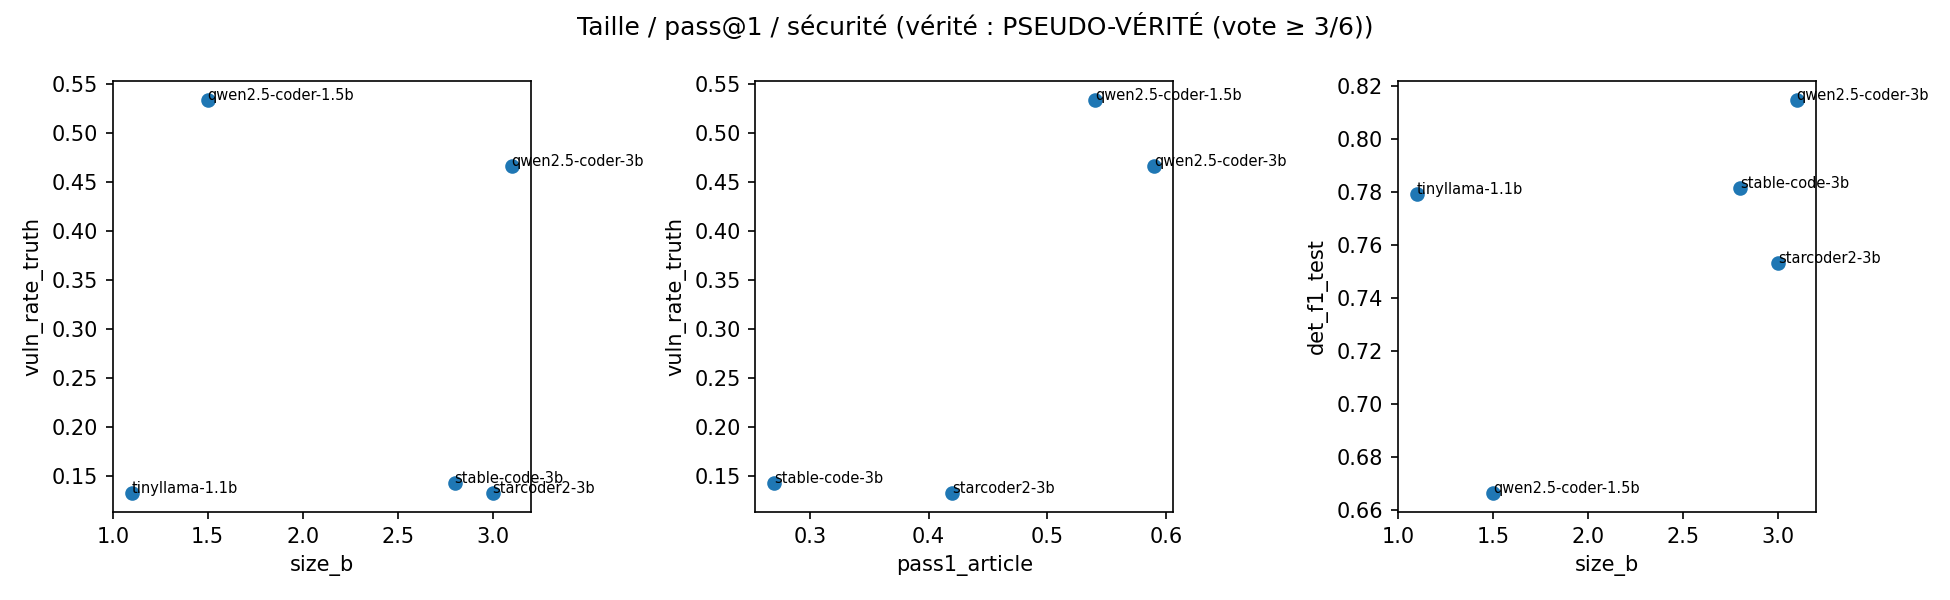
\includegraphics[width=0.95\linewidth]{size_security.png}
\caption{Taille, pass@1 et sécurité (vérité : pseudo-vérité, vote $\geq 3/6$)}
\label{fig:size}
\end{figure}

Aucune corrélation n'est significative avec quatre ou cinq modèles. Aucune ne va cependant dans le sens \og plus grand ou plus performant = plus sûr \fg : Qwen2.5-Coder 3B, meilleur pass@1 (0,59), présente le taux de vulnérabilité Bandit le plus élevé (40\,\%), et TinyLlama (1,1 B), une fois affiné, détecte aussi bien que les modèles de 3 milliards de paramètres.

\section{Profils de compétences}
\begin{figure}[H]
\centering
\begin{subfigure}[b]{0.56\linewidth}
  \centering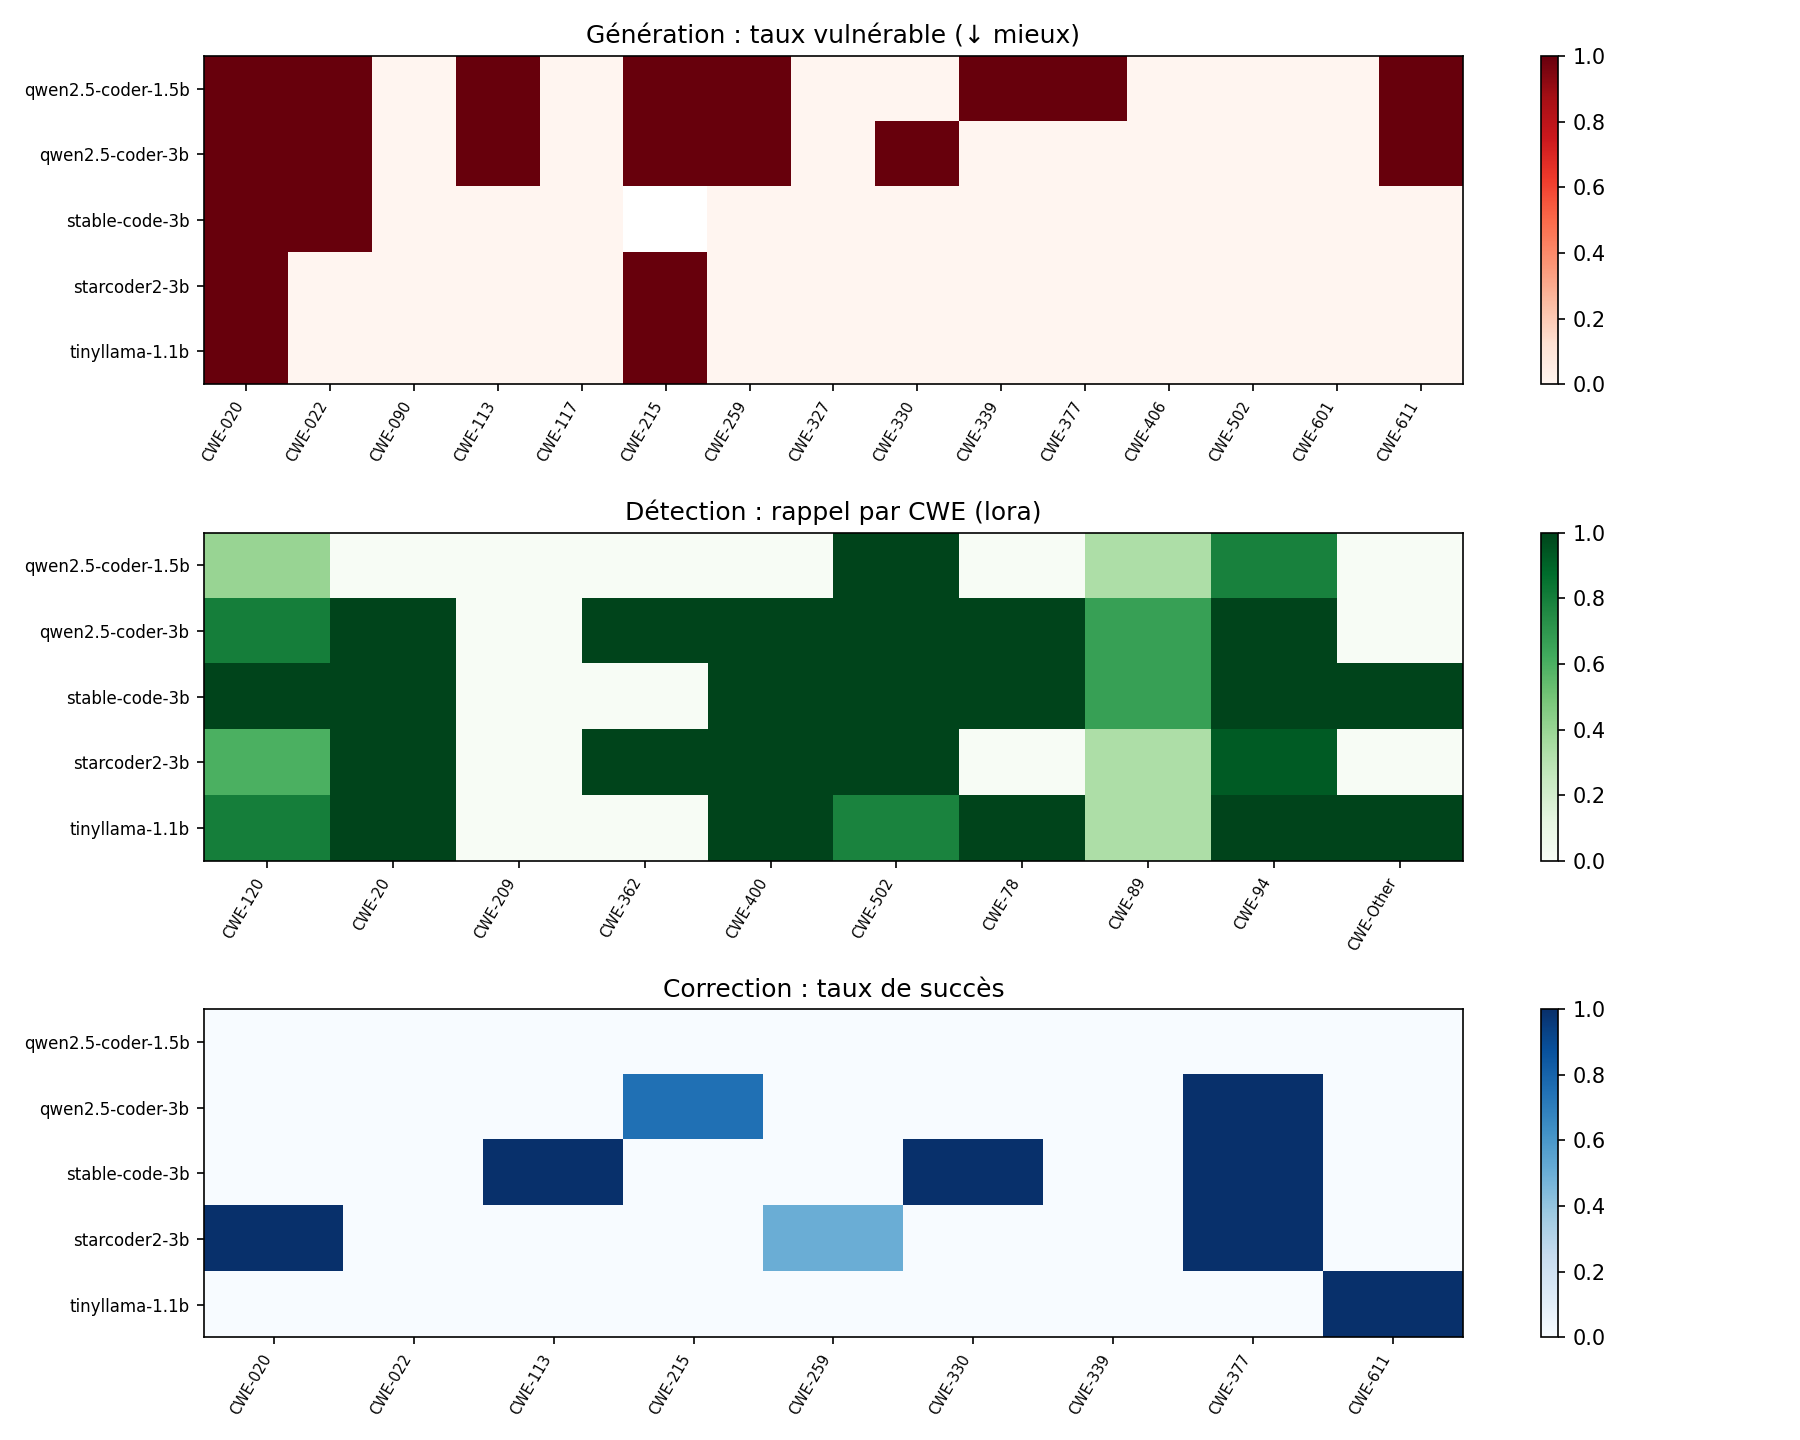
\includegraphics[width=\linewidth]{profil_heatmap.png}
  \caption{Par modèle et par CWE}
\end{subfigure}\hfill
\begin{subfigure}[b]{0.42\linewidth}
  \centering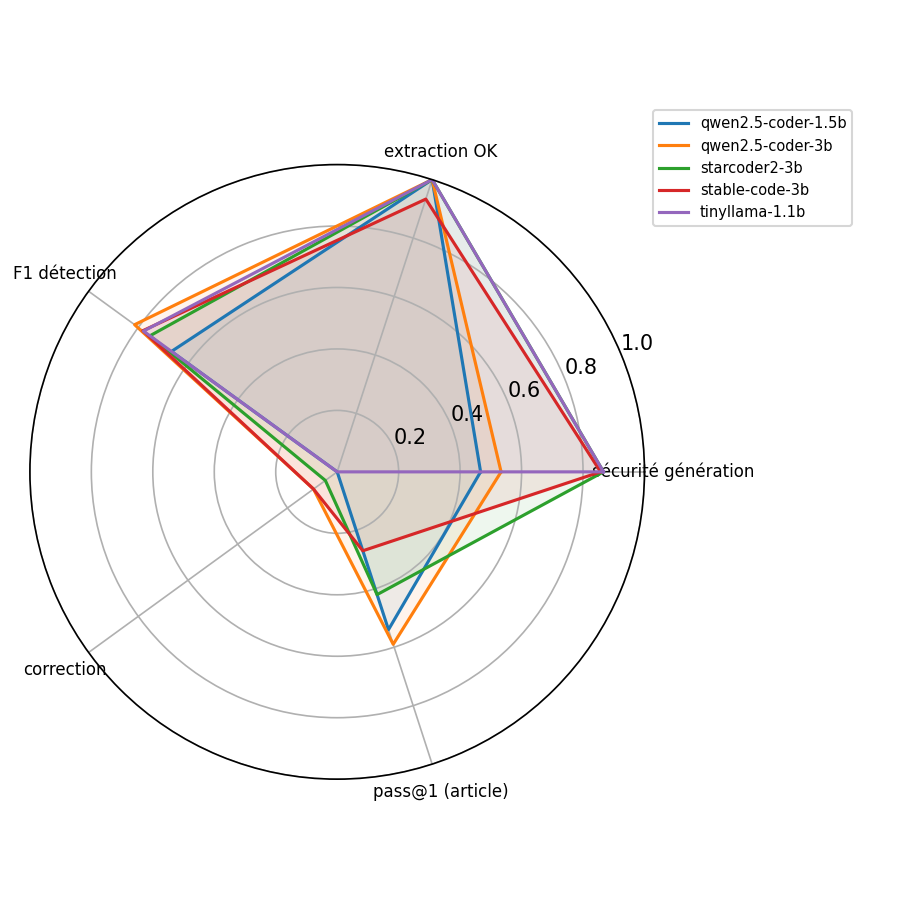
\includegraphics[width=\linewidth]{profil_radar.png}
  \caption{Synthèse par modèle}
\end{subfigure}
\caption{Profils de compétences : génération, détection et correction}
\label{fig:profils}
\end{figure}

% =====================================================================
\chapter{Discussion, limites et perspectives}\label{chap:discussion}
% =====================================================================

\section{Interprétation}
\begin{description}[style=nextline]
  \item[Génération] Près d'un code sur trois est vulnérable, principalement par reproduction d'API courantes mais dangereuses. La qualité fonctionnelle mesurée par pass@1 ne protège pas de ces failles.
  \item[Détection] Un affinage QLoRA léger suffit à transformer un SLM en détecteur plus performant que Bandit, capable en outre d'identifier la bonne catégorie de faille. C'est le résultat le plus encourageant de l'étude : un détecteur local, peu coûteux et explicable.
  \item[RAG] Le RAG n'est pas un gain automatique : sans entraînement adapté au contexte, il perturbe le détecteur.
  \item[Correction] La correction automatique reste peu fiable, et les contrôles automatiques surestiment fortement sa réussite : une relecture humaine est indispensable.
\end{description}

\section{Limites}
\begin{itemize}
  \item \textbf{Taille d'échantillon} : 15 prompts et une réponse par prompt ; les écarts entre générateurs ne sont pas statistiquement robustes.
  \item \textbf{Pseudo-vérité} : sur les codes générés, la vérité est un vote des détecteurs, donc biaisée en leur faveur ; le fichier d'annotation humaine est prêt mais n'a pas été rempli.
  \item \textbf{Jeu d'entraînement} : CyberNative est petit (594 exemples) et synthétique, et ses CWE sont déduites par mots-clés ; les scores sur le test surestiment probablement la performance sur du code réel.
  \item \textbf{RAG absent de l'entraînement} : il explique la dégradation des configurations LoRA + RAG.
  \item \textbf{Bandit} : il repère des motifs d'appels mais ignore les failles logiques et le flux des données.
  \item \textbf{Pas de tests fonctionnels} : la préservation du comportement des corrections n'est vérifiée que par la relecture humaine.
  \item \textbf{pass@1} : il provient d'un autre protocole, et TinyLlama n'y figure pas.
\end{itemize}

\section{Perspectives}
\begin{itemize}
  \item Annoter manuellement les 74 codes générés pour disposer d'une vérité indépendante.
  \item Générer plusieurs réponses par prompt pour des taux statistiquement solides.
  \item Entraîner les détecteurs avec le contexte RAG.
  \item Utiliser un jeu d'entraînement plus réaliste, issu de vulnérabilités réelles.
  \item Ajouter des tests unitaires pour valider le comportement des corrections.
  \item Étendre l'étude à d'autres langages de programmation.
\end{itemize}

% =====================================================================
\chapter{Conclusion}\label{chap:conclusion}
% =====================================================================
Ce projet a évalué cinq SLMs open source dans trois rôles complémentaires. Il montre que :
\begin{enumerate}
  \item \textbf{les SLMs génèrent du code vulnérable} dans \chiffre{29,7\,\%} des cas, et un meilleur score fonctionnel ne garantit pas un code plus sûr ;
  \item \textbf{un SLM affiné par QLoRA}, en quelques minutes sur un GPU gratuit, détecte les vulnérabilités \textbf{mieux que Bandit} (F1 jusqu'à \chiffre{0,81} contre 0,64) et identifie mieux leur catégorie ;
  \item \textbf{la correction automatique reste peu fiable} : \chiffre{4,8\,\%} seulement des tentatives aboutissent à une correction réellement valide, et la validation automatique ne détecte pas la plupart des fausses corrections.
\end{enumerate}
En résumé, \textbf{un SLM peut surveiller le code, mais pas encore le réparer seul}. Un détecteur local, léger et explicable est à portée de main, à condition de conserver un humain dans la boucle pour la correction.

% =====================================================================
\appendix
\chapter{Reproduction des expériences}
\section{Organisation du dépôt}
\begin{tabularx}{\linewidth}{@{}lX@{}}
\toprule
\code{slmsec.py} & bibliothèque commune \\
\code{notebooks/00 à 06} & une phase par notebook Google Colab \\
\code{results/} & tableaux CSV et figures produits par les notebooks \\
\code{presentation/} & présentation de soutenance (HTML) et mode présentateur \\
\code{rapport/} & ce rapport (\LaTeX) \\
\bottomrule
\end{tabularx}

\section{Ordre d'exécution}
\begin{enumerate}
  \item Copier \code{slmsec.py} dans \code{MyDrive/slm-security/}.
  \item Exécuter dans l'ordre les notebooks 00 (configuration), 01 (génération), 02 (Bandit), 03 (détecteurs), 04 (benchmark), 05 (correction) et 06 (extras).
  \item Chaque étape enregistre ses résultats sur Drive et saute ce qui existe déjà : un notebook interrompu peut être relancé.
\end{enumerate}

% =====================================================================
\begin{thebibliography}{99}
\addcontentsline{toc}{chapter}{Bibliographie}

\bibitem{hasan} M.~M.~Hasan, M.~Waseem, K.-K.~Kemell, J.~Rasku, J.~Ala-Rantala et P.~Abrahamsson. \emph{Assessing small language models for code generation: An empirical study with benchmarks}. The Journal of Systems \& Software, 2026.

\bibitem{securityeval} M.~L.~Siddiq et J.~C.~S.~Santos. \emph{SecurityEval dataset: mining vulnerability examples to evaluate machine learning-based code generation techniques}. Proceedings of the 1st International Workshop on Mining Software Repositories Applications for Privacy and Security (MSR4P\&S), 2022.

\bibitem{cybernative} CyberNative. \emph{Code\_Vulnerability\_Security\_DPO} (jeu de données). Hugging Face, \url{https://huggingface.co/datasets/CyberNative/Code_Vulnerability_Security_DPO}.

\bibitem{cwe} MITRE. \emph{Common Weakness Enumeration (CWE)}. \url{https://cwe.mitre.org}.

\bibitem{bandit} PyCQA. \emph{Bandit — security linter for Python}. \url{https://github.com/PyCQA/bandit}.

\bibitem{lora} E.~J.~Hu, Y.~Shen, P.~Wallis, Z.~Allen-Zhu, Y.~Li, S.~Wang, L.~Wang et W.~Chen. \emph{LoRA: Low-Rank Adaptation of Large Language Models}. International Conference on Learning Representations (ICLR), 2022.

\bibitem{qlora} T.~Dettmers, A.~Pagnoni, A.~Holtzman et L.~Zettlemoyer. \emph{QLoRA: Efficient Finetuning of Quantized LLMs}. Advances in Neural Information Processing Systems (NeurIPS), 2023.

\bibitem{rag} P.~Lewis et al. \emph{Retrieval-Augmented Generation for Knowledge-Intensive NLP Tasks}. Advances in Neural Information Processing Systems (NeurIPS), 2020.

\bibitem{bge} S.~Xiao, Z.~Liu, P.~Zhang et N.~Muennighoff. \emph{C-Pack: Packaged Resources To Advance General Chinese Embedding} (modèles BGE). arXiv:2309.07597, 2023.

\bibitem{faiss} J.~Johnson, M.~Douze et H.~Jégou. \emph{Billion-scale similarity search with GPUs}. IEEE Transactions on Big Data, 2019.

\bibitem{transformers} T.~Wolf et al. \emph{Transformers: State-of-the-Art Natural Language Processing}. Proceedings of EMNLP: System Demonstrations, 2020.

\end{thebibliography}

\end{document}
